% Created 2016-08-17 Wed 14:38
\documentclass[tikz]{standalone}

\usepackage[utf8]{inputenc}
\usepackage[T1]{fontenc}

\usepackage{circledsteps}

\RequirePackage{xcolor}

%% HPI color definitions according to the design manual
% These do not exactly match the RGB values used in the Powerpoint slide master due to unknown reasons
\definecolor{hpiyellow}{RGB}{246,168,0}
\definecolor{hpiorange}{RGB}{221,97,8}
\definecolor{hpired}{RGB}{177,6,58}
\definecolor{hpigray}{RGB}{90,96,101}
\definecolor{hpiblue}{RGB}{0,122,158}


\renewcommand{\sfdefault}{neosans}
% Different font weights for neosans
\newcommand{\textl}[1]{{\fontseries{l}\selectfont #1}} % light
\newcommand{\textm}[1]{{\fontseries{m}\selectfont #1}} % medium, same as default weight
\newcommand{\textsb}[1]{{\fontseries{sb}\selectfont #1}} % semibold
\newcommand{\textmb}[1]{{\fontseries{mb}\selectfont #1}} % bold, same as \textbf
\newcommand{\texteb}[1]{{\fontseries{eb}\selectfont #1}} % extra bold
\newcommand{\textub}[1]{{\fontseries{ub}\selectfont #1}} % ultra bold

\tikzset{every picture/.style={/utils/exec={\sffamily}}}
\tikzset{flipflop RSflanke/.style={
  flipflop,
  flipflop def={t1=S, t2=C, c2=1, t3=R, t6=Q, t4={\ctikztextnot{Q}}}
}}


\tikzset{
  mechanicalSwitch/.pic={
    \coordinate (-inUp) at (135:2); 
    \coordinate (-inDown) at (235:2);
    \coordinate (-out) at (2,0);
    \coordinate (-center) at (0,0);
    
    \draw (0,0) circle [radius = 2cm];
    \draw [fill=gray!20] (0,0) circle [radius = 0.2cm];

    \draw (0, 0) -- (2, 0);
    \draw (135:.8) -- (135:2); 
    \draw (225:.8) -- (225:2); 

    \draw [fill=gray!20] (2, 0) circle [radius=0.05cm]; 
    \draw [fill=gray!20] (135:2) circle [radius=0.05cm]; 
    \draw [fill=gray!20] (225:2) circle [radius=0.05cm]; 

    
    \draw [thick] (0,0) -- (175:1.5); 

    \draw [dashed, <->, domain=135:225] plot ({cos(\x)}, {sin(\x)}); 
  },
  mechanicalSwitchClosed/.pic={
    \coordinate (-inUp) at (135:2); 
    \coordinate (-inDown) at (255:2);
    \coordinate (-out) at (2,0);
    \coordinate (-center) at (0,0);
    \draw (0,0) circle [radius = 2cm];
    \draw [fill=gray!20] (0,0) circle [radius = 0.2cm];

    \draw (0, 0) -- (2, 0);
    \draw (135:.8) -- (135:2); 
    \draw (225:.8) -- (225:2); 

    \draw [fill=gray!20] (2, 0) circle [radius=0.05cm]; 
    \draw [fill=gray!20] (135:2) circle [radius=0.05cm]; 
    \draw [fill=gray!20] (225:2) circle [radius=0.05cm]; 

    
    \draw [thick] (0,0) -- (135:2); 

    \draw [dashed, <->, domain=135:225] plot ({cos(\x)}, {sin(\x)}); 
  }
}


\usetikzlibrary{calc}
\usetikzlibrary{positioning}


\usetikzlibrary{ext.positioning-plus,chains,backgrounds,shapes.multipart}


\begin{document}

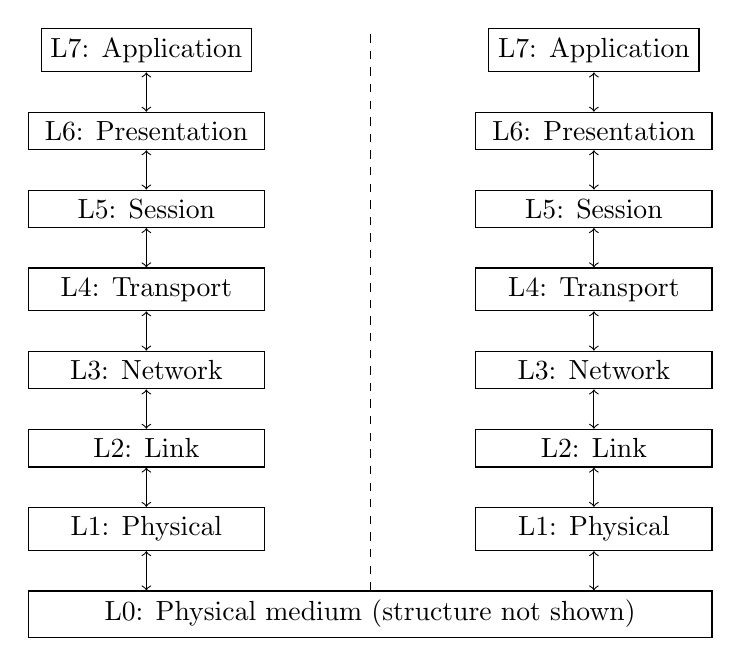
\begin{tikzpicture}[start chain=1 going below, start chain=2 going below,
  node distance=0.5cm,
  every join/.style=<->
  ]

  \label{page:basics:reference:iso:twonodes}
  
  \node [on chain =1, draw, ] (l7l) {L7: Application};
  \node [on chain =2, draw, right=3cm of l7l] {L7: Application};
  
  \foreach \n/\k [count=\i] in {6/Presentation, 5/Session, 4/Transport, 3/Network, 2/Link, 1/Physical}{
    \node [on chain=1, draw, minimum width=3cm, join] (ll\i) {L\n: \k}; 
    \node [on chain=2, draw, minimum width=3cm, join] (lr\i) {L\n: \k}; 
  }

  \node [below=of -(ll6) (lr6), draw] (l0) {L0: Physical medium (structure not shown)}; 
  \draw [<->] (ll6) -- (l0.north -| ll6);
  \draw [<->] (lr6) -- (l0.north -| lr6);
  \draw [dashed] (l0.north) -- (l0.north |- l7l.north) ; 
\end{tikzpicture}

% TODO: fix numbering of nodes with respect to layers! 
\newcommand{\sevenlayers}[0]{  \node [on chain =1, ] (l7l) {L7: Application};
  \node [on chain =4, right=11cm of l7l] (l7r) {L7: Application};
  
  \foreach \n/\k [count=\i] in {6/Presentation, 5/Session, 4/Transport, 3/Network, 2/Link, 1/Physical}{
    \node [on chain=1] (ll\i) {L\n: \k}; 
    \node [on chain=4] (lr\i) {L\n: \k}; 
  }

  \node [on chain=2, right=2cm of ll4] (lrouter3) {L3: Network};
  \node [on chain=2] (lrouter2) (lrouter2) {L2: Link};
  \node [on chain=2] (lrouter1) (lrouter1) {L1: Physical};

  \node [on chain=3, right=2cm of lrouter2] (lswitch2) {L2: Link};
  \node [on chain=3] (lswitch1) {L1: Physical};
  

  \node [below=of -(ll6) (lr6), draw] (l0) {L0: Physical medium (structure not shown)}; 
  \draw [<->] (ll6) -- (l0.north -| ll6);
  \draw [<->] (lr6) -- (l0.north -| lr6);
  \draw [<->] (lrouter1) -- (l0.north -| lrouter1);
  \draw [<->] (lswitch1) -- (l0.north -| lswitch1);
  % \draw [dashed] (l0.north) -- (l0.north |- l7l.north) ;

  \begin{scope}[every path/.style=dotted]
    \coordinate (tmp) at ($(ll6)!0.5!(lrouter1)$);
    \draw (tmp |- l0.north) -- (tmp |- l7l.north); 
    \coordinate (tmp) at ($(lrouter1)!0.5!(lswitch1)$);
    \draw (tmp |- l0.north) -- (tmp |- l7l.north); 
    \coordinate (tmp) at ($(lswitch1)!0.5!(lr5)$);
    \draw (tmp |- l0.north) -- (tmp |- l7l.north); 
  \end{scope}
}

\begin{tikzpicture}[start chain=1 going below, start chain=2 going below,
  start chain=3 going below, start chain=4 going below,
  node distance=0.5cm,
  every node/.style={draw, minimum width=3cm, join},
  every join/.style=<->
  ]

  \label{page:basics:reference:iso:fournodes}

  \sevenlayers
\end{tikzpicture}

\newcommand{\logicalcomm}[0]{  \begin{scope}[every path/.style = <->, dashed, thick]
    \foreach \l/\r in { l7l/l7r, ll1/lr1, ll2/lr2, ll3/lr3, ll4/lrouter3,
      lrouter3/lr4, ll5/lrouter2, lrouter2/lswitch2, lswitch2/lr5,
      ll6/lrouter1, lrouter1/lswitch1, lswitch1/lr6} { \draw (\l) -- (\r); }
  \end{scope}
}

\begin{tikzpicture}[start chain=1 going below, start chain=2 going below,
  start chain=3 going below, start chain=4 going below,
  node distance=0.5cm,
  every node/.style={draw, minimum width=3cm, join},
  every join/.style=<->
  ]

  \label{page:basics:reference:iso:logical}

  \sevenlayers
  \logicalcomm 
  
\end{tikzpicture}

\begin{tikzpicture}[start chain=1 going below, start chain=2 going below,
  start chain=3 going below, start chain=4 going below,
  node distance=0.5cm,
  every node/.style={draw, minimum width=3cm, join},
  every join/.style=<->
  ]

  \label{page:basics:reference:iso:groups}

  \sevenlayers
  \logicalcomm

  \begin{scope}[on background layer]
    \node [draw=hpiyellow, fill=hpiyellow!5, rounded corners, fit=(l7l)(l7r)(ll3)(lr3)]  (e2ebox) {};
    \node [left=of e2ebox, rotate=90,draw=none,anchor=south] {\textbf{End-to-end layers}};
    
    \node [draw=hpiorange, fill=hpiorange!5, rounded corners, fit=(ll4)(lr4)(ll6)(lr6)] (networkbox) {};
    \node [left=of networkbox, rotate=90,draw=none, anchor=south] {\textbf{Network layers}};
    
    \node [draw=hpiblue, fill=hpiblue!5, rounded corners, fit=(lr5)(lr6)(lrouter2)] (networkbox) {};
    \node [right=of networkbox, rotate=270, draw=none, anchor=south] {\textbf{Link layers}};
    
  
  \end{scope}
  
\end{tikzpicture}

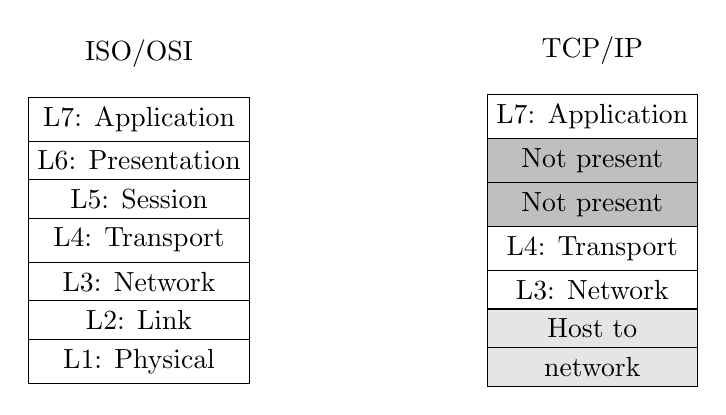
\begin{tikzpicture}
  \label{page:arch:reference:osi_vs_tcp}
  
  \node [draw, rectangle split, rectangle split parts=7,] (isoosi) {
    L7: Application 
    \nodepart{two} L6: Presentation
    \nodepart{three} L5: Session 
    \nodepart{four} L4: Transport 
    \nodepart{five} L3:  Network
    \nodepart{six} L2:  Link
    \nodepart{seven} L1: Physical 
  };

  \node [above=0.25 of isoosi] {ISO/OSI}; 

  \node [draw, right=3cm of isoosi,
  rectangle split, rectangle split parts=7,
  rectangle split part fill={white,gray!50, gray!50, white, white, gray!20, gray!20},
  ] (tcpip) {
    L7: Application 
    \nodepart{two} \emph{Not present} 
    \nodepart{three} \emph{Not present} 
    \nodepart{four} L4: Transport 
    \nodepart{five} L3:  Network
    \nodepart{six} Host to 
    \nodepart{seven} network
  };

  \node [above=0.25 of tcpip] {TCP/IP}; 

  
  % TODO: get rid of the line in TCP/IP between two lower layers? 

  
\end{tikzpicture}


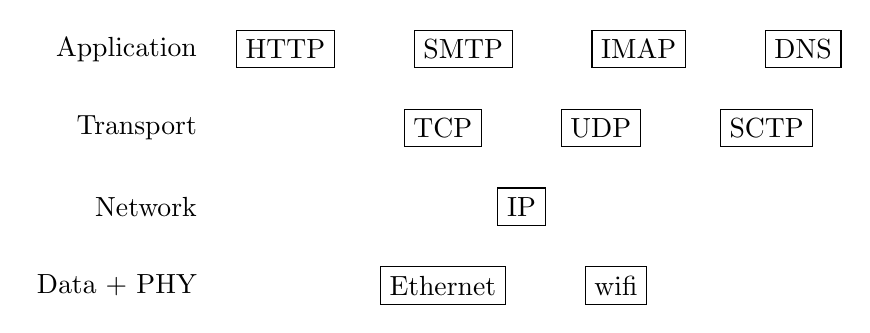
\begin{tikzpicture}[every node/.style=draw]
  \label{page:arch:hourglass}

  % application
  \node at (-2, 4) (http) {HTTP};
  \node [right=of http] (smtp) {SMTP}; 
  \node [right=of smtp] (imap) {IMAP}; 
  \node [right=of imap] (dns) {DNS};

  \node at (0,3) (tcp) {TCP}; 
  \node [right= of tcp] (udp) {UDP}; 
  \node [right= of udp] (sctp) {SCTP};

  \node at (1,2) (ip) {IP};

  \node at (0,1) (ether) {Ethernet};
  \node [right = of ether] (wifi) {wifi};
  % \node [right = of wifi] {Optical Fibre}; 

  \begin{scope}[every node/.style={draw=none,anchor=east}]
    \node at (-3,4) {Application}; 
    \node at (-3,3) {Transport}; 
    \node at (-3,2) {Network}; 
    \node at (-3,1) {Data + PHY}; 
  \end{scope}


\end{tikzpicture}

\begin{tikzpicture}
  \label{page:arch:reference:merged}
  \node [draw, right=3cm of isoosi,
  rectangle split, rectangle split parts=5,
  % rectangle split part fill={white, white, white, gray!20, gray!20},
  ] (tcpip) {
    L7: Application 
    \nodepart{two} L4: Transport 
    \nodepart{three}L3:  Network 
    \nodepart{four}  L2: Data link 
    \nodepart{five} L1: PHY  
  };

  \node [above=0.25 of tcpip] {Merged ISO/OSI \& TCP/IP}; 

  
  % TODO: get rid of the line in TCP/IP between two lower layers? 

  
\end{tikzpicture}



\end{document} 